\chapter{Representing Information with Symbols}
\label{chapter:representingInformationWithWymbols}

\section{Similar Words}
\label{section:similarWords}

Representing information with symbols is a fundamental concept of Computer Science as information should be represented clear and concisely. Words can be seen as a sequence of symbols, namely a sequence of letters.

\subsection{Exercises}

Transmitting information includes representing it in a message, sending it to the destination and the receiver being able to make sense of it even tough the message might contain errors such as a spelling mistake. To achieve this sender and receiver agree to only send messages with a minimal editing distance \cite{AnD} between each of them. 

The editing distance is the amount of operations that need to be done to transform a message in another. Operations are deleting, inserting and changing a letter \TODO{add some TI explanation}. A cost function exists that defines the cost of each operation, and in our case each operation has a cost of 1 (unit cost model). The editing distance is then the minimal cost to transform a message into another one by a sequence of operations. In our case a message is a word.

\begin{example}
    The editing distance between \code{LIKE} and \code{BIKE} is 1, since changing the first letter from an \code{L} to and \code{B} transforms the first word into the second.
\end{example}

If sender and receiver agree to only transmit words with a minimal editing distance of e.g 3, then the receiver can still uniquely determine what word the sender has sent even when at most 1 spelling mistake has been made. The receiver calculates the minimal editing distance between the received word and each of the agreed words and chooses the word with the least editing distance.
The receiver assume that this was the word the sender wanted to sent. This of course work only if there are not more than 1 error in the word. If this happens the editing distance to another word is closer than to the original word and hence the word is misinterpreted. To counter this, sender and receiver might agree on a bigger minimal distance, but this comes with a tradeoff. When chosing a bigger minimal distance for a fixed alphabet, the number of words that can be used shrinks. To maintain the same amount of words the size of the alphabet can be increased too, resulting in longer words.

The purpose of the \nameref{section:similarWords} exercises is to learn these operations. Therefore an exercise is dedicated to each opertion: adding, changing and removing a letter from a word. Additionally, an exercise about swapping adjacent letters in a word is included. Swapping adjacent letters is not part of the mentioned operations and usually consists of 2 operations: removing and adding or changing twice. However, when typing on a keyboard typing mistakes happen often and most of the time only two adjacent letters are swapped. This exercises is supposed to train the ability to spot these sort of mistakes.

\subsection*{Adding a letter}

In the \code{adding a letter} exercise pupils are presented a word, the alphabet from A to Z and spaces between each letter of the word as well as at the beginnig and the end of the word, where a letter can be added. Pupils are supposed to choose a letter from the alphabet and add it to one of the mentioned spaces to form a new valid word.

\begin{example}
    The word \code{PACE} is given. By adding the letter \code{S} before the first letter, the valid word \code{SPACE} is formed.
\end{example}

\subsection*{Changing a letter}

In this exercise there is again a word and the alphabet from A to Z shown. Again pupils should select a letter from the alphabet, but this time, instead of adding it to a space, the selected letter should be replace a letter from the word itself to create a new valid word.

\begin{example}
    The word \code{BIKE} is given. By changing the first letter from a \code{B} to a \code{L} the new valid word \code{LIKE} is formed.
\end{example}

\subsection*{Removing a letter}

In this exercise pupils receive a word and they should select a character from within the word an move it to the trashcan to remove the letter from the word itself to form a new valid word.

\begin{example}
    The word \code{SPACE} is given. By removing the first letter the new valid word \code{PACE} is formed.
\end{example}

\subsection*{Swapping adjacent letters}

To learn to recognize typing mistakes in a word pupils are presented a word with swapped adjacent letters and they are supposed to identify those and swap them back to restore to original word. Here are multiple difficulty levels possible, where on the easy level only one pair of adjacent letters is swapped and on harder levels multiple pairs of adjacent letters are swapped.

\begin{example}
    The word \code{BKIE} is given. By swapping the second and third letter the original word \code{BIKE} is restored.
\end{example}

\subsection{Implementation}

\subsection*{Word Generation}

The foundation of these exercises is to have a list of words and for each word a list of similar words. A similar word is a word to which the original word can be transformed to by either adding, changing or removing a letter. Generating a list of words is the easy part. Basically any list of words will do the jobs, but they should be understable for pupils. So the first step is to collect a list of nouns for children provided by a online service \cite{}. 

Not much more difficult, but much more expensive is the computation of similar word. Given the children nouns list and the allowed words list, one can brute force a list of similar word by simply applying each transformation to every children noun and checking whether the transformed word exists in the allowed word lists. The script to generate a list of similar words for each word and each operation is given in listing \ref{lst:similarWords}. To have multiple difficulty levels in the exercise \code{Changing Letters}, similar word with an editing distance of two are generated as well. All other operations only include words with an editing distance of one.

%TC:ignore
\begin{lstlisting}[language=Python,caption={Algorithm to generate a list of similar words},label={lst:similarWords}]
for word in children_words:
  add = list()
  for pos in range(len(word) + 1):
    for letter in ALPHABET:
      w = word[:pos] + letter + word[pos:]
      if contains(allowed_words, w) and not w in add:
        add.append(w.upper())
  similar_words["add"][1][word.upper()] = add

  remove = list()
  for pos in range(len(word)):
      w = word[:pos] + word[pos + 1 :]
      if contains(allowed_words, w) and not w in remove:
          remove.append(w.upper())
  similar_words["remove"][1][word.upper()] = remove

  change = list()
  for pos in range(len(word)):
    for letter in ALPHABET:
      w = word[:pos] + letter + word[pos + 1 :]
      if w != word and contains(allowed_words, w) and not w in change:
        change.append(w.upper())
  similar_words["change"][1][word.upper()] = change

  change = list()
  for left_pos in range(len(word)):
    for right_pos in range(left_pos + 1, len(word)):
      for left_letter in ALPHABET:
        for right_letter in ALPHABET:
          if word[left_pos] == left_letter or word[right_pos] == right_letter:
            continue
          w = (
            word[:left_pos]
            + left_letter
            + word[left_pos + 1 : right_pos]
            + right_letter
            + word[right_pos + 1 :]
          )
          if w != word and contains(allowed_words, w) and not w in change:
            change.append(w.upper())
  if len(change) >= MIN_SIMILAR_WORDS:
    change.sort()
    similar_words["change"][2][word.upper()] = change
\end{lstlisting}
%TC:endignore

\begin{example}
  Examples of similar words for adding, changing and removeing a letter from a word
  \begin{itemize}
    \item \textbf{adding a letter} - arm: arme, arms, darm, farm, warm
    \item \textbf{changing a letter} - buch: auch, bach, bush, euch, huch, such, tuch
    \item \textbf{removing a letter} - bauch: auch, bach, buch
  \end{itemize}
\end{example}

There is no need to generate a list of similar word for the \code{Swapping letters} exercise, since the letters can be swapped during the exercise creation.
\TODO{maybe check for editing distances}

Significantly more difficult is to generate a list of allowed words. Three different approaches were taken:

\begin{itemize}
  \item Using a list of approximately ten thousand nouns
  \item Collecting a list from online dictionary of allowed words of the well known word game Scrabble \cite{Scrabble}
  \item Generating a list from a spell checker
\end{itemize}

The first approach resulted in having a word list with which exercises could be generated. However, the word list obviously did not cover all possible word pupils could find. Therefore the word list needed to be extended.

Hence the idea to collect Scrabble word came up. This seemed like a good idea until it showed that the online Scrabble dictionary did also not contain all valid words.
Collecting words from the Scrabble dictionary resulted in approximately thirty thousand word between two and 8 charachters long.

Finally, the last approach was taken by generating a list of allowed word from a spell checker. However, spell checkers do not have a list of all allowed word, but rather of two files: the dictionary file and the affix file. The dictionary files contains a list of words and applicable rules for each word and the affix file contains a list explaining these rules. Each rule defines a prefix or suffix that can be applied to a word \cite{Hunspell}. 
\TODO{example of dictionary and affix file}
Luckily there exists a tool called \code{unmunch} in the hunspell ecosystem that generates a list of words from the dictionary file and the affix file as easy as shown in listing \ref{lst:unmunch} \cite{HunspellGithub}.
In the end a list of about one million allowed words was generated (without any word length limits). However, a drawback is that the wordlist does not contain any names from people, cities or any other instances. 

%TC:ignore
\begin{lstlisting}[language=Bash,caption={Bash command to unmunch a dictionary file and a affix file to a list of wird},label={lst:unmunch}]
$ unmunch German_de_CH.dic German_de_CH.aff > wordlist.txt
\end{lstlisting}
%TC:endignore

\TODO{add pictures}
The actual implementation of these exercise types is now pretty straigh forward. Basically, each type has a word displayed, split up by each letter to allow easy user interaction. Two exercise types, namely adding and changing a letter, need an alphabet and hence make use of the \code{ItemSelection.vue} component. The ''adding a letter'' exercise is implemented in the \code{Add.vue} component and shows arrow between each letter and at the beginning and end of the word, where pupils can add a new letter selected from the alphabet. The ''change a letter'' exercise work similarly, but instead of having arrows, pupils can change each letter itself with a new letter selected from the alphabet. In the ''remove a letter'' exercise pupils can move a letter to the trashcan to remove it and in the ''swap letters' exercise they can click on the arrows to change the order of the letters. Additionally, this exercise has another difficulty level, where two letter pairs are swapped instead of only one.

\section{Number Systems}
\label{section:numberSystems}
\TODO{add pictures}

\subsection{Exercises}
\subsection*{Representing Numbers like the Maya}

Today, one is used to the decimal number system (base number 10), with 10 symbols. The Maya used a different number system with with a base number of 20 i.e the vigesimal number system. It is believed that the Maya used their ten fingers and ten toes to count adding up to twenty. But instead of having a symbol for each number as in the decimal system, the Maya used three different symbols: zero (a turtle shell, belly side up), one (a dot) and five (a bar) \cite{Maya}. The mayan representation of the decimal number from 0 to 19 can be found in figure \ref{fig:maya_numerals}.

\begin{figure} 
    \centering
    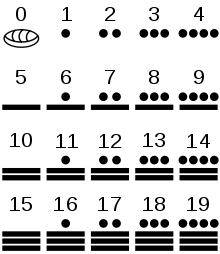
\includegraphics[width=0.3 \columnwidth]{figures/maya_number_system.png}
    \caption{Representation of the Maya numbers from 0 to 19} 
    \label{fig:maya_numerals} 
\end{figure}

The following exercises are supposed to familiarize pupils with a new number system, the mayan number system. First converting numbers between the decimal number system and the mayan numbers is trained topped of an exercise about adding two mayan numbers.

\subsubsection*{Representing mayan numbers}

A decimal number is presented to the pupils and they need to choose the correct amount of dots and bars representing the decimal number. For the purpose of simplicity, only decimal numbers between 1 and 19 are chosen.

\begin{example}
    The decimal number \code{17} is writte as three bars and two dots.
\end{example}

\subsubsection*{Understanding mayan numbers}

In this exercise the pupils learn to understand mayan numbers. Again only decimal numbers between 1 and 19 are used and the pupils need to understand what mayan number is shown and write down the decimal equivalent.

\subsubsection*{Adding mayan numbers}

To sum this section up, adding mayan numbers is learned. This exercises combines the previous two, since the pupils need to understand the summands given in the mayan number system, add them and write the sum down in either decimal number system or the mayan number system.

\subsection*{Representing Numbers with Coins}

The following exercises introduce a new number system and trains an already learned one: the binary number system and the decimal number system. Both number systems are praticed with coins with numbers. The binary coins include the following numbers: 1, 2, 4, 8, 16, 32 and 64 (figure \ref{fig:binary_coins}). The decimal coins include 1, 2, 5, 10, 20 and 50 (figure \ref{fig:decimal_coins}). 
Overall, the same concepts are praticed for both number systems with the limitation that every binary coin can at most be used once. For both number systems the following exercises are given:
\begin{itemize}
    \item Conversion of a decimal number to its coin representation
    \item Conversion of a number given in its coin representation to a decimal number
\end{itemize}
Additionally, for the decimal number system the following exercise is given:
\begin{itemize}
    \item Reducing the number of decimal coins in a given set of decimal coins
\end{itemize}

\begin{figure} 
    \centering
    
\includegraphics[width=0.5 \columnwidth]{figures/decimal_coins.png}
    \caption{Representation of the decimal coins} 
    \label{fig:decimal_coins} 
\end{figure}

\begin{figure} 
    \centering
    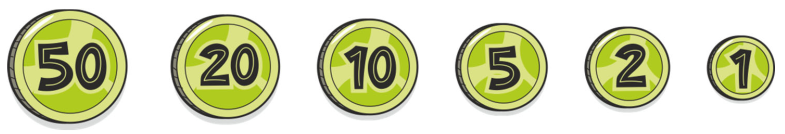
\includegraphics[width=0.5 \columnwidth]{figures/binary_coins.png}
    \caption{Representation of the binary coins} 
    \label{fig:binary_coins} 
\end{figure}

\subsubsection*{Conversion of a decimal number to its coin representation}

This exercise includes two difficulty levels:
\begin{itemize}
    \item Converting a decimal number to a coin representation, where the sum of all coins are equal to the decimal number
    \item Converting a decimal number to a coin representation, where the sum of all coins are equal to the decimal number \textbf{and} the amount of used coins is minimal.
\end{itemize}

\subsubsection*{Conversion of a number given in its coin representation to a decimal number}

This exercise is straigh forward. A number given in its coin representation, either binary or decimal coins, have to be converted to a decimal number. 

\subsubsection*{Reducing the amount of decimal coins in a given set of decimal coins}

Similar to the previous exercise, a number in its coin representation is given and pupils have to display the same number but with less coins.

\subsection{Implementation}

The conversion exercises from the decimal number system \textbf{to} either the mayan, decimal coins or binary coins all share the same logic implemented in the \code{To.vue} component.
The same goes for the inverse direction (\code{From.vue} component).
However, adding mayan numbers (\code{Addition.vue}) and reducing the amount of used coins (\code{Swap.vue}) have their own logic. 

The \code{To.vue} component is simple. It shows a a random number between 1 and a number system specific limit:

\begin{itemize}
  \item \textbf{Mayan number system} - limit: 19
  \item \textbf{Decimal coins} - limit: 100
  \item \textbf{Binary coins} - limit: 100
\end{itemize}

The pupils need to select items (either nuts, sticks or coins) with the correct value and place it so these items sum up to the shown random number.
Additionally for the the convertion to the decimal coins, there is another difficulty level asking to represent the shown random number with as few decimal coins as possible. To algorithm to calculate the minimal amount of items necessary for a certain sum is given in listing \ref{lst:calcMinimalAmount} 


%TC:ignore
\begin{lstlisting}[language=TypeScript,caption={Calculate minimal amount of items needed to reach a certain number},label={lst:calcMinimalAmount}]
calcMinimalAmount(type: numbersystemType, number: number): number[] {
  const items = this.items(type);
  let i = 0;
  const minimalAmount = new Array<number>(items.length).fill(0);
  while (number > 0 && i < items.length) {
    const value = items[i].value;
    if (number >= value) {
      minimalAmount[i]++;
      number -= value;
    } else {
      i++;
    }
  }
  return minimalAmount;
}
\end{lstlisting}
%TC:endignore

The implementation for the \code{From.vue} component works in a similar fashion. This time a random amount of each item is generated. \TODO{maybe show these limits} The pupils finally need to add the values of these items up.

Both of these components need at some point to sum the values items. It would be convenient to have a map where each item type maps to the amount of selected respectively shown item and a map where each item type maps to its value. However, due to Vue.js constraints this is not possible since maps are not reactive. \TODO{introduce reactivity}
Arrays on the other hand are. Therefore an array is used, having the first element to be the highest item value, down to the last element being the item with the lowest value. This introduces some thight coupling between the array storing the amount of items and the array storing the value of each item. The implementation to sum item is shown in listing \ref{lst:sumItems}.

%TC:ignore
\begin{lstlisting}[language=TypeScript,caption={Sum up items},label={lst:sumItems}]
sumItems(type: numbersystemType, items: number[]): number {
  if (items.length !== this.items(type).length) {
    throw Error(`array lengths do not match:  ${items} ${this.items(type)}`);
  }
  let sum = 0;
  for (let i = 0; i < this.items(type).length; i++) {
    sum += items[i] * this.items(type)[i].value;
  }
  return sum;
}
\end{lstlisting}
%TC:endignore

The \code{Swap.vue} component reuses some parts of the just mentioned components. It also generates a random amount of each item. The total amount of items is reducable and pupils are asked to represent the same sum over all items but with fewer items. How such a configuration is achieved, is shown in listing \ref{lst:reducableItems}.

%TC:ignore
\begin{lstlisting}[language=TypeScript,caption={Generate a reducable item configuration},label={lst:reducableItems}]
do {
  this.generatedItems = this.generateItems(this.type);
} while (
  this.sumItems(this.type, this.generatedItems) >= this.limit(this.type) ||
  this.countItems(this.generatedItems) ===
    this.countItems(
      this.calcMinimalAmount(
        this.type,
        this.sumItems(this.type, this.generatedItems)
      )
    )
);
\end{lstlisting}
%TC:endignore

In the \code{Addition.vue} component all previously seen concepts come together. Two summands are generated, each having a random amount of items. The sum is guaranteed to not overshoot the limit of this number system. This exercise has two difficulty levels:

\begin{itemize}
  \item \textbf{easy} - the pupils have to calculate the sum as a number 
  \item \textbf{medium} - the puils have to calculate the sum as a representation of items
\end{itemize}
